\documentclass[paper=letter, fontsize=12pt]{article}
\usepackage{geometry}
\geometry{margin=1in}
\usepackage{graphicx}
\graphicspath{{images/}}
\usepackage{amssymb}

%opening
\title{Compsci 571 HW1}
\author{Yilin Gao (yg95)}

\begin{document}

\maketitle

\section{Perceptron Algorithm and Convergence Analysis}

\begin{enumerate}
\item Perceptrons can be used to represent many Boolean functions $f: \{0, 1\} \rightarrow \{0, 1\}$ in n-dimensional space.
\begin{enumerate}
	\item Provide a two-input Boolean function $y = f(x_1, x_2)$, where $y, x_1, x_2 \in \{0, 1\}$, that can be represented by a single perceptron. Plot the points $(x_1, x_2)$ that represent all possible pair values (e.g. (0, 0), (0, 1), (1, 0), (1, 1)) and provide a separating hyperplane on the same figure.
	
	\textbf{Answer:}
	
	The function $y$ can be:
	
	\begin{tabular} {|c|c|c|}
		\hline
		$y$ & $x_1$ & $x_2$	\\ \hline
		0 & 0 & 0 \\ \hline
		1 & 0 & 1 \\ \hline
		1 & 1 & 0 \\ \hline
		1 & 1 & 1 \\ \hline
	\end{tabular} \\

	One possible separating hyperplane can be: $f(x_1, x_2) = x_1 + x_2 - 0.5$. 
	
	Plot: 
	
	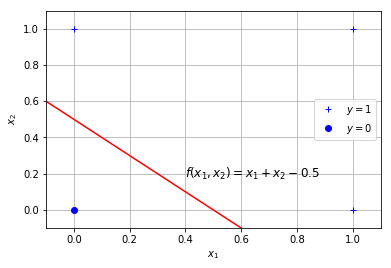
\includegraphics[scale=0.5]{1a.png}
	
	\item Provide a two-point Boolean function $y = f(x_1, x_2)$ that cannot be represented by a single perceptron. Briefly explain why.
	
	\textbf{Answer:}
	
	The function $y$ can be:
	
	\begin{tabular} {|c|c|c|}
		\hline
		$y$ & $x_1$ & $x_2$	\\ \hline
		0 & 0 & 0 \\ \hline
		1 & 0 & 1 \\ \hline
		1 & 1 & 0 \\ \hline
		0 & 1 & 1 \\ \hline
	\end{tabular} \\

	This is because these data are not linearly separable (in this case, fully separated by a line). According to the properties of Perceptron algorithm, if the training data are not linearly separable, the algorithm will fail.
	
	\item Provide a three-input Boolean function $y = f(x_1, x_2, x_3)$, where $y, x_1, x_2, x_3 \in \{0, 1\}$, that can be represented by a single perceptron. Plot the points $(x_1, x_2, x_3)$ that represent all possible pair values and provide a separating hyperplane on the same figure.
	
	\textbf{Answer:}
	
	The function $y$ can be:
	
	\begin{tabular} {|c|c|c|c|}
		\hline
		$y$ & $x_1$ & $x_2$	& $x_3$\\ \hline
		0 & 0 & 0 & 0\\ \hline
		0 & 1 & 0 & 0 \\ \hline
		0 & 0 & 0 & 1 \\ \hline
		0 & 1 & 0 & 1 \\ \hline
		1 & 0 & 1 & 0\\ \hline
		1 & 1 & 1 & 0 \\ \hline
		1 & 0 & 1 & 1 \\ \hline
		1 & 1 & 1 & 1 \\ \hline
	\end{tabular} \\

	One possible separating hyperplane can be: $f(x_1, x_2, x_3) = x_2 - 0.5$
	
	Plot:
	
	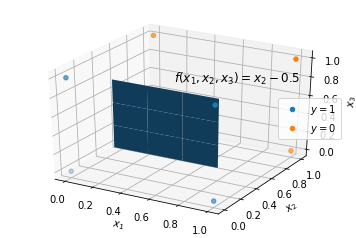
\includegraphics[scale=0.6]{1c.png}
	
\end{enumerate}

\item For a response variable $y \in \{-1, 1\}$ and a linear classification function $f(x) = \beta_0 + \beta^T x$, suppose that we classify according to $sign(f(x))$. Show that the signed Euclidean Distance of the point $x$ with label $y$ to the decision boundary is given by $\frac{1}{\Vert\beta\Vert_2}yf(x)$.

\textbf{Answer:}

According to the definition of Euclidean Distance of a point $x$ to a line $f(x) = 0$, unsigned (positive) Euclidean Distance $ = \frac{1}{\sqrt{\beta_1^2 + \dots + \beta_n^2}} f(x) = \frac{1}{\Vert \beta \Vert_2} f(x)$ .

If $y = 1$, signed Euclidean Distance = unsigned Euclidean Distance $= \frac{1}{\Vert \beta \Vert_2} f(x) = \frac{1}{\Vert \beta \Vert_2} yf(x)$.

If $y = -1$, signed Euclidean Distance = negative unsigned Euclidean Distance $= \frac{1}{\Vert \beta \Vert_2} (-f(x))= \frac{1}{\Vert \beta \Vert_2} yf(x)$.

So in both cases, the signed Euclidean Distance of the point $x$ with label $y$ the the decision boundary $f(x)$ is $\frac{1}{\Vert\beta\Vert_2}yf(x)$. 

\item Suppose we have $n$ points $x_i \in \mathbb{R}^p$ with class labels $y_i \in \{-1, 1\}$. Points are correctly classified by a hyperplane $w^{sep^T}x = 0$, $\Vert w^{sep} \Vert_2 \leq 1$. Assuming $y_i w^{sep^T}x_i \geq 1$ for all $i$ and $\max_i \Vert x_i \Vert_2 = 1$, show that the perceptron algorithm converges to a separating hyperplane in no more than $\Vert w^{(0)} - w^{sep} \Vert^2_2$ steps.

\textbf{Answer:}

Assume the perceptron algorithm converges to the separating hyperplane in $T$ steps.

First, 
\begin{equation}
(\vec{w}^{sep} \cdot \vec{w}^{t}) - (\vec{w}^{sep} \cdot \vec{w}^{t-1}) = y_i (\vec{w}^{sep} \cdot \vec{x_i})
\end{equation}
\begin{equation}
\geq 1
\end{equation}
\begin{equation}
\vec{w}^{sep} \cdot \vec{w}^{T} - \vec{w}^{sep} \cdot \vec{w}^{0} = \sum_{t=0}^{T-1} [(\vec{w}^{sep} \cdot \vec{w}^{t}) - (\vec{w}^{sep} \cdot \vec{w}^{t-1})] \geq T
\end{equation}
\begin{equation}
\vec{w}^{sep} \cdot\vec{w}^{T} \geq T + \vec{w}^{sep} \cdot \vec{w}^{0}
\end{equation}

Step (1) is proven in class. Step (2) is given in the question.

Second,
\begin{equation}
\Vert \vec{w}^{t} \Vert^2 = \Vert \vec{w}^{t-1} + y_i \vec{x_i} \Vert^2 = \Vert \vec{w}^{t-1} \Vert^2 + 2y_i(\vec{w}^t \cdot \vec{x_i}) + y_i^2 \Vert \vec{x_i} \Vert^2
\end{equation}
\begin{equation}
\leq \Vert \vec{w}^{t-1} \Vert^2 + 1
\end{equation}
\begin{equation}
\Vert \vec{w}^{T} \Vert^2 \leq \Vert \vec{w}^{0} \Vert^2 + T
\end{equation}

Step (5) is proven in class. Step (6) is because for the misclassified point $i$ its margin $y_i(\vec{w}^t \cdot \vec{x_i}) \leq 0$, $y_i^2 = 1$ and $\Vert \vec{x_i} \Vert_2 \leq 1$.

Third,
\begin{equation}
\Vert \vec{w}^{T} - \vec{w}^{sep} \Vert^2 = \Vert \vec{w}^{sep} \Vert^2 + \Vert \vec{w}^{T} \Vert^2 - 2 * \vec{w}^{sep} \cdot \vec{w}^{T}
\end{equation}
\begin{equation}
\leq \Vert \vec{w}^{sep} \Vert^2 + \Vert \vec{w}^{0} \Vert^2 + T - 2 * (\vec{w}^{sep} \cdot \vec{w}^0 + T)
\end{equation}
\begin{equation}
= \Vert \vec{w}^0 - \vec{w}^{sep} \Vert^2 - T
\end{equation}

So,
\begin{equation}
T \leq \Vert \vec{w}^0 - \vec{w}^{sep} \Vert^2 - \Vert \vec{w}^{T} - \vec{w}^{sep} \Vert^2 \leq \Vert \vec{w}^0 - \vec{w}^{sep} \Vert^2 \ \ \ \square
\end{equation}
Step (9) is to plug in the results of steps (4) and (7). Step (11) is because $\Vert \vec{w}^{T} - \vec{w}^{sep} \Vert^2 \geq 0$.

\end{enumerate}

\section{Programming Assignment}

\textbf{For questions 1 and 2, if not stated otherwise, the epoch parameter is set to 100. And for initial data processing, I preserved the original data order from MNIST.}

\begin{enumerate}
\item 
\begin{enumerate}
	\item 
	The plot between epoch counter and the algorithm accuracy on training set:
	
	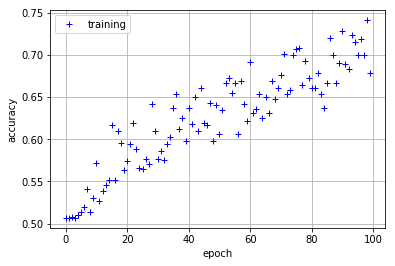
\includegraphics[scale=0.5]{p2q1a.png}
	
	As the epoch counter increases, the accuracy doesn't have an evident increasing or decreasing tendency.
	
	So if I increase the maximum number of epochs, the accuracy after the algorithm finishes will keep around the current level. If the perceptron algorithm is able to separate points perfectly, the accuracy will finally reach 1. If I decrease the maximum number of epochs, the accuracy after the algorithm finishes will also keep around the current level.
	
	\item 
	The plot between epoch counter and the algorithm accuracy on both training and testing data:
	
	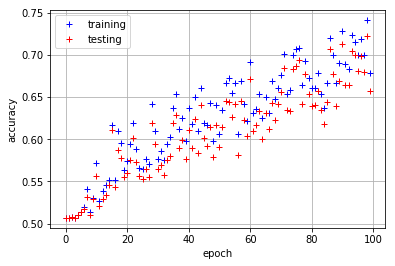
\includegraphics[scale=0.5]{p2q1b.png}
	
	Same as on the training data, as the epoch counter increases, the accuracy doesn't have an evident increasing or decreasing tendency.
	
	Compare to the plot on training data, the perceptron weights have lower accuracy on testing data. This indicates the algorithm overfits a bit on the training data.
	
	\item 
	The accuracy of the perpeptron algorithm on the testing data after the last epoch is 0.9598191863385234.
	
	The confusion matrix is:
	
	\begin{tabular} {|c|c|c|}
		\hline
		 & Actual yes: $y = +1$ & Actual no: $y = -1$	\\ \hline
		Predicted yes: $\hat{y} = +1$& 943 & 41 \\ \hline
		Predicted no: $\hat{y} = -1$ & 39 & 968 \\ \hline
	\end{tabular}

	\item 
	The ROC curves on training data with $w'$ and $w*$ are:
	
	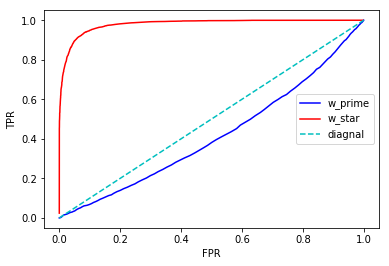
\includegraphics[scale=0.5]{p2q1d.png}
	
	The ROC curve depicts the trade off relationship between FPR (cost of the algorithm) and TPR (benefit of the algorithm), i.e., for a given FPR, what's the value of TPR. For a given FPR, we would prefer a higher TPR. Because $w*$ leads to a ROC curve higher than $w'$,  $w*$ stands for a better decision boundary than $w'$.
	
	\item
	AUC for $w*$ is 0.9958677813010872.
	 
	AUC for $w'$ is 0.988769684392598.
	
	AUC is the area under the ROC between $FPR = 0$ and $FPR = 1$. So if ROC reaches higher values more quickly, its corresponding AUC is larger. The approximated AUCs for two curves are pretty close to each other, while AUC of $w*$ is a little bit larger, which is consistent with their ROC shapes. The larger AUC of $w*$ also indicates $w*$ leads to a better decision boundary.
	 
\end{enumerate}

\item 
\begin{enumerate}
	\item 
	The plot between epoch counter and the algorithm accuracy on training data is:
	
	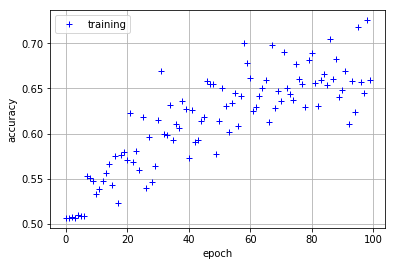
\includegraphics[scale=0.5]{p2q2a.png}
	
	The accuracy of the balanced winnow algorithm on the testing data is 0.9663485685585133.
	
	The confusion matrix on the testing data is:
	
	\begin{tabular} {|c|c|c|}
		\hline
		& Actual yes: $y = +1$ & Actual no: $y = -1$	\\ \hline
		Predicted yes: $\hat{y} = +1$& 954 & 39 \\ \hline
		Predicted no: $\hat{y} = -1$ & 28 & 970 \\ \hline
	\end{tabular}

	\item 
	In question 2(a) I set $\eta = 0.1$. Now I try out $\eta = [0.2, 0.3, 0.4, 0.5]$, and compute the relationship between epoch counter and algorithm accuracy for each $\eta$. From the following plot, I find out that among the five values, $\eta = 0.1$ (the blue line) has the best performance in terms of algorithm accuracy.
	
	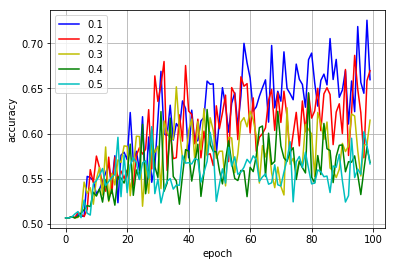
\includegraphics[scale=0.5]{p2q2b1.png}
	
	This is also the case when I set $I = 500$:
	
	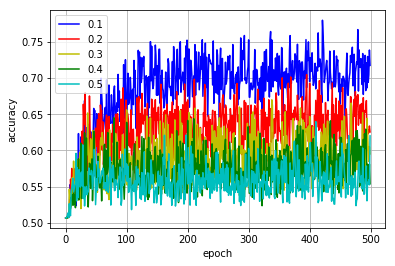
\includegraphics[scale=0.5]{p2q2b3.png}
	
	After this, I try $\eta = [0.02, 0.04, 0.06, 0.08]$ to see if smaller values would lead to even better accuracy. From the following plot where $I = 100$, I think the performances of $\eta = [0.02, 0.04, 0.06, 0.08, 0.1]$ are similar to each other.
	
	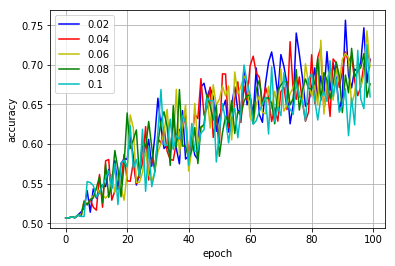
\includegraphics[scale=0.5]{p2q2b2.png}
	
	This is also the case when I set $I = 500$:
	
	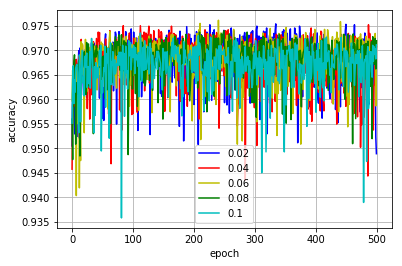
\includegraphics[scale=0.5]{p2q2b4.png}
	
	So based on my experiments, when $I = 100$ and $I = 500$, $\eta = [0.02, 0.04, 0.06, 0.08, 0.1]$ work better than larger values in terms of accuracy.
	
	In general, to tune a parameter in an algorithm, I would try to use as many values of the parameter as possible, calculate certain reasonable measuring metrics of the algorithm under each parameter value, and see if some parameter values can lead to better performance of these measuring metrics. 
	
	And also I would consider the joint effect of the target parameter and other parameters. It's likely that when other parameters take different values, the optimized target parameter is also different.
\end{enumerate}
\end{enumerate}

\end{document}
